% !TeX root = ../../Book4.tex
% 纲要标题：## 第15章　滤过复形与谱序列
% 纲要标签：b4:ch:14
% 纲要位置：计划纲要.md，第 3586 行。

\chapter{滤过复形与谱序列}
\label{b4:ch:14}
\BookChapterNumber{b4:ch:14}

\begin{chapterabstract}
本章从滤过复形构造谱序列的各页与微分，在逐度有限条件下证明收敛，并借双复形例子区分高阶微分和稳定页后的扩张问题。
\end{chapterabstract}

\begin{learninggoals}
\begin{itemize}
\item 固定递减滤过和上同调型指标，核对 \(\mathrm{d}_r\) 的次数。
\item 用代表元修正推导各页以及页间同调关系。
\item 检查逐度有限条件，说明稳定页与上同调滤过的关系，并构造正合偶及其导出。
\item 判断哪些微分可能非零，计算一个非零 \(\mathrm{d}_2\)，正确使用边缘同态。
\item 区分高阶微分与稳定页后的扩张问题。
\end{itemize}
\end{learninggoals}

设域 \(k\) 上的双复形只有 \(C^{0,1}=ka\)、\(C^{1,0}=kb\)、\(C^{1,1}=kc\)、\(C^{2,0}=ke\) 四个非零项，非零箭头为 \(\mathrm{d}_ha=c\)、\(\mathrm{d}_vb=c\)、\(\mathrm{d}_hb=e\)。按列先取上同调，只剩 \([a]\) 和 \([e]\)，两者之间没有第一阶微分；可是总复形从次数一到次数二的微分矩阵是 \(\left(\begin{smallmatrix}1&1\\0&1\end{smallmatrix}\right)\)，总上同调为零。后面构造谱序列时，要找出究竟是哪一个微分消去了这两个类；\secref{b4:sec:1405}会完成计算。

\ProseParagraphBreak
本章需要\chapref{b4:ch:05}的上同调长正合列和\chapref{b4:ch:06}的反交换双复形、总化约定。\chapref{b4:ch:13}的逆极限解释了为什么无界收敛另有困难。复合函子与群扩张的例子将在下一章使用这里建立的有限滤过谱序列。

\ProseParagraphBreak
阅读材料可选 Weibel 的《An Introduction to Homological Algebra》\cite[Sections 5.2--5.5, Section 5.9]{Weibel1994HomologicalAlgebra}。其中谱序列的分次记号先以同调型给出，本章直接采用后面复合函子所需的上同调型约定。关于稳定页后的结构恢复，应同时回顾\chapref{b4:ch:09}中短正合列与一次 Ext 的联系。

% !TeX root = ../../Book4.tex
% 纲要标题：### 15.1 滤过与伴随分次
% 纲要标签：b4:sec:1401
% 纲要位置：计划纲要.md，第 2827 行。

\section{滤过与伴随分次}
\label{b4:sec:1401}

滤过先把复形分成较简单的层，再保留微分在层间移动的信息。递增与递减编号会改变后面公式的方向，有界、穷尽与分离条件也必须分别说明。

% 纲要内容：
%
% * 递增、递减滤过
% * 有界、穷尽和分离条件
% * 首先固定指标方向
%

\subsection{递增滤过与递减滤过}
\label{b4:subsec:1401:01}

把一个复杂复形分成几层，往往比直接求核再求商容易。例如双复形的总次数固定以后，可以先保留横指标较大的那些项。微分可能把一层送到更深的一层；若暂时忽略这种移动，便得到一组较简单的复形。谱序列记录随后怎样把这些层间信息逐步补回来。

\begin{definition}\label{b4:def:filtered-complex}
设 \(\mathcal A\) 为交换范畴，\(C\) 为 \(\mathcal A\) 中的上链复形。对每个整数 \(p\)，给定子复形 \(F^pC\subseteq C\)，若
\[
 F^{p+1}C\subseteq F^pC,
\]
则称 \((C,F)\) 为带\term[dijian-lvguo]{递减滤过}[decreasing filtration]的复形。其\term[bansui-fenci]{伴随分次}[associated graded object]为复形族
\[
 \operatorname{gr}_F^pC=F^pC/F^{p+1}C.
\]
若改用 \(F_pC\subseteq F_{p+1}C\)，则得到递增滤过。滤过映射 \(f:(C,F)\to(D,F)\) 是满足 \(f(F^pC)\subseteq F^pD\) 的复形映射。
\end{definition}

用 \(F^pC=F_{-p}C\) 可以互换递增、递减记号，但微分的指标也必须相应改变。本章固定递减约定。若 \(D^{a,b}\) 是第一象限双复形，令
\[
 F^p\operatorname{Tot}(D)^n=\bigoplus_{a\ge p}D^{a,n-a}.
\]
纵微分保持 \(a\)，横微分增大 \(a\)，所以总微分保持这个子对象。伴随分次只剩第 \(p\) 列，最先显现的是纵向上同调。

章首四项双复形的中间列 \(kb\xrightarrow{1}kc\) 正合，左右两列各留下一个类。按列取上同调看到的这两个类仍不足以给出总上同调；横向微分怎样穿过已经正合的中间列，正是后续页要记录的信息。

\subsection{有界、穷尽与分离条件}
\label{b4:subsec:1401:02}

\begin{definition}\label{b4:def:finite-filtration}
设 \(\mathcal A\) 为交换范畴，\((C,F)\) 为 \(\mathcal A\) 中的递减滤过上链复形。若对每个总次数 \(n\) 存在整数 \(a_n<b_n\)，使 \(F^{a_n}C^n=C^n\)、\(F^{b_n}C^n=0\)，则称滤过逐度有限。若 \(a_n,b_n\) 可独立于 \(n\) 选取，则称滤过一致有界。

若对每个 \(n\)，子对象族 \((F^pC^n)_{p\in\mathbb Z}\) 的和（包含序中的最小公共上界）存在且等于 \(C^n\)，则称滤过穷尽；若各次的交（最大公共下界）存在且等于零子对象，则称滤过分离。对模而言，嵌套子模的和就是并，所以这两个条件分别写成 \(\bigcup_pF^pC^n=C^n\) 与 \(\bigcap_pF^pC^n=0\)。
\end{definition}

逐度有限时，每次滤过已经包含全对象与零子对象，上述和与交自动存在，因此蕴含穷尽和分离；它不要求复形只有有限多个次数。第一象限双复形的列滤过在总次数 \(n\ge0\) 满足 \(F^0=C^n\)、\(F^{n+1}=0\)，就是本书最常用的逐度有限情形。

\ProseParagraphBreak
穷尽和分离本身不保证有限计算。例如 \(C^0=\mathbb Z\)、其他次数为零，取 \(F^pC^0=2^p\mathbb Z\)（\(p\ge0\)）、\(F^pC^0=\mathbb Z\)（\(p<0\)），便得到穷尽、分离但不逐度有限的滤过。商群 \(C^0/F^pC^0\) 的相容系统还包含并非来自某个整数的元素。因此讨论无限滤过时，是否需要完备化是实质问题；本章的主要收敛定理采用逐度有限条件，不把这些差别省去。

\subsection{滤过的指标方向}
\label{b4:subsec:1401:03}

总次数写作 \(n=p+q\)，其中 \(p\) 是滤过次数，\(q\) 只是补足总次数的第二指标。在模的情形，一个 \(x\in F^pC^{p+q}\) 若满足 \(\mathrm{d}x\in F^{p+r}C^{p+q+1}\)，便表示它的微分直到相隔 \(r\) 层才可能被看见。于是第 \(r\) 次出现的微分必须具有方向
\[
 \mathrm{d}_r:E_r^{p,q}\longrightarrow E_r^{p+r,q-r+1}.
\]
它使总次数增加一；在第零页竖直向上，在第一页水平向右，第二页向右两格、向下一格。\cref{b4:fig:spectral-differential-directions}将前四种方向放在同一网格中比较。

\begin{figure}[htbp]
\centering
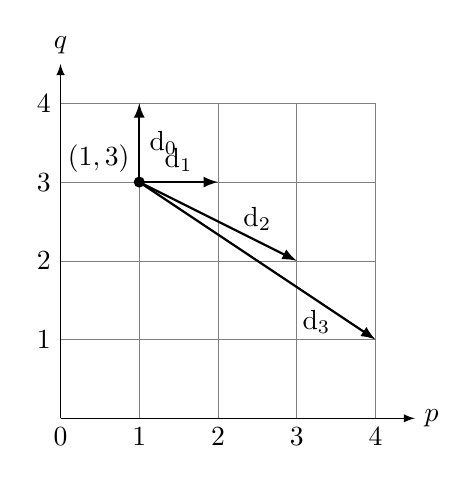
\begin{tikzpicture}[x=1cm,y=1cm,>=latex]
\draw[help lines] (0,0) grid (4,4);
\draw[->] (0,0)--(4.5,0) node[right]{\(p\)};
\draw[->] (0,0)--(0,4.5) node[above]{\(q\)};
\foreach \i in {0,1,2,3,4}
  \node[below] at (\i,0){\(\i\)};
\foreach \j in {1,2,3,4}
  \node[left] at (0,\j){\(\j\)};
\fill (1,3) circle (2pt);
\node[above left] at (1,3){\((1,3)\)};
\draw[->,thick] (1,3)--(1,4) node[midway,right]{\(\mathrm d_0\)};
\draw[->,thick] (1,3)--(2,3) node[midway,above]{\(\mathrm d_1\)};
\draw[->,thick] (1,3)--(3,2) node[pos=0.75,above]{\(\mathrm d_2\)};
\draw[->,thick] (1,3)--(4,1) node[pos=0.75,below]{\(\mathrm d_3\)};
\end{tikzpicture}
\caption[上同调型谱序列的微分方向]{上同调型谱序列的微分方向。以 \((1,3)\) 为示意源，四支箭头分别表示不同页的位移 \((0,1)\)、\((1,0)\)、\((2,-1)\)、\((3,-2)\)。}
\label{b4:fig:spectral-differential-directions}
\end{figure}

\begin{definition}\label{b4:def:spectral-sequence}
设 \(\mathcal A\) 为交换范畴。给定 \(\mathcal A\) 中的双分次对象 \(E_r^{p,q}\)，其中 \(r\ge0\)、\(p,q\in\mathbb Z\)，以及态射 \(\mathrm{d}_r:E_r^{p,q}\to E_r^{p+r,q-r+1}\)。若这些态射及指定同构满足
\[
 \mathrm{d}_r^2=0,\qquad E_{r+1}^{p,q}\simeq
 \frac{\ker(\mathrm{d}_r:E_r^{p,q}\to E_r^{p+r,q-r+1})}
 {\operatorname{im}(\mathrm{d}_r:E_r^{p-r,q+r-1}\to E_r^{p,q})}
\]
则称这些数据构成从第零页开始的上同调型\term[pu-xulie]{谱序列}[spectral sequence]。也可从某个较晚页开始给出这些数据。谱序列态射在各页保持双次数、与微分及指定同构相容。
\end{definition}
\symidx{\(E_r^{p,q},\mathrm{d}_r\)：谱序列的页与微分}

这个定义描述的是一列反复取上同调的对象，尚未指定它计算什么。目标及其滤过必须另外给出；不能只凭写出 \(E_2\) 就宣称已经算出某个上同调群。下面从实际滤过复形构造全部各页，再证明它们与原复形上同调的关系。

% !TeX root = ../../Book4.tex
% 纲要标题：### 15.2 谱序列的构造
% 纲要标签：b4:sec:1402
% 纲要位置：计划纲要.md，第 2833 行。

\section{谱序列的构造}
\label{b4:sec:1402}

第零页只看伴随分次，后续微分则测量代表元还能向深层提升多少次。本节先从代表元直接构造各页，再证明每一新页由前一页取同调得到。

% 纲要内容：
%
% * E_0、E_1 及微分
% * 页间同调关系
%

\subsection{\texorpdfstring{\(E_0\)、\(E_1\) 与微分}{E0、E1 与微分}}
\label{b4:subsec:1402:01}

设 \(\mathcal A\) 为交换范畴，\((C,F)\) 为 \(\mathcal A\) 中的递减滤过上链复形。第零页为
\[
 E_0^{p,q}=F^pC^{p+q}/F^{p+1}C^{p+q},\qquad \mathrm{d}_0[x]=[\mathrm{d}x].
\]
微分保持滤过，保证它良定义。因此
\[
 E_1^{p,q}=H^{p+q}(F^pC/F^{p+1}C).
\]
若 \(x\) 代表此页的类，便有 \(\mathrm{d}x\in F^{p+1}\)。再取 \(\mathrm{d}x\) 在下一层的类，就得到 \(\mathrm{d}_1[x]\)。

\ProseParagraphBreak
例如，取零次和一次的两项复形 \(C=(\mathbb Z\xrightarrow{2}\mathbb Z)\)，并令 \(F^pC=C\)（\(p\le0\)）、\(F^1C=(0\to\mathbb Z)\)、\(F^pC=0\)（\(p\ge2\)）。乘 \(2\) 把源的滤过层零送入靶的滤过层一，所以伴随分次上的 \(\mathrm{d}_0\) 为零。第零页与第一页都只有两个非零项，但第一页微分恢复了原复形中跨过一层滤过的映射：
\[
 E_1^{0,0}=\mathbb Z\xrightarrow{\ \mathrm{d}_1=\times2\ }
 E_1^{1,0}=\mathbb Z.
\]
于是第二页只剩 \(E_2^{1,0}=\mathbb Z/2\)，以后再无可能的非零微分。它与 \(H^0(C)=0\)、\(H^1(C)=\mathbb Z/2\) 相符：先逐层看时得到的两个自由群，通过后续微分才合成为原复形的挠同调。

\ProseParagraphBreak
为同时写出后面各页，令 \(n=p+q\)，并对 \(r\ge0\) 定义
\[
 Z_r^{p,q}=F^pC^n\cap \mathrm{d}^{-1}(F^{p+r}C^{n+1}).
\]
这里子对象的交通过两嵌入的拉回定义，\(\mathrm d^{-1}(F^{p+r}C^{n+1})\) 是沿微分的拉回原像；两个子对象的和是它们的直和映入 \(C^n\) 所得的像。每页的公式只涉及有限交、有限和及商对象。特别地 \(Z_0^{p,q}=F^pC^n\)。当 \(r\ge1\) 时，置
\begin{equation}\label{b4:eq:spectral-page-formula}
 E_r^{p,q}=
 \frac{Z_r^{p,q}}
 {Z_{r-1}^{p+1,q-1}+\mathrm{d}Z_{r-1}^{p-r+1,q+r-2}}.
\end{equation}
分母第一项容许更改较深一层的代表元，但其微分也要足够深；第二项容许减去已经可见的余边。两项确实包含于分子：第一项的微分位于 \(F^{p+r}\)，第二项位于 \(F^p\) 且再次微分为零。取 \(r=1\)，公式正是上面第零页的上同调。

\subsection{页间同调关系}
\label{b4:subsec:1402:02}

\begin{theorem}\label{b4:thm:filtered-spectral-sequence}
设 \(\mathcal A\) 为交换范畴，\((C,F)\) 为 \(\mathcal A\) 中的递减滤过上链复形。取 \(E_0^{p,q}=F^pC^{p+q}/F^{p+1}C^{p+q}\)，并对 \(r\ge1\) 以\cref{b4:eq:spectral-page-formula}定义 \(E_r^{p,q}\)。原复形的微分诱导 \(\mathrm d_r:E_r^{p,q}\to E_r^{p+r,q-r+1}\)，其代表元公式为 \(\mathrm{d}_r[x]=[\mathrm{d}x]\)。这些页构成谱序列，且对滤过复形映射自然。
\end{theorem}
\begin{proof}
以下记 \(n=p+q\)。在模范畴中可以直接作代表元计算；一般情形按\cref{b4:lem:generalized-element-calculus}使用广义元素。记号 \(x\in Z\) 表示一个态射 \(x:T\to Z\)，\([x]\) 表示其经商态射所得的像。从商对象选代表、从像中选原像，或把子对象和中的态射写成两个分量之和时，都先沿相应满态射的拉回预合成。有限次操作可取共同的满态射细化，下面仍沿用原符号；同一等式内的态射具有相同的定义域，态射等式最终可消去预合成的满态射。

第零页微分的核在 \(F^pC^n\) 中的原像是 \(Z_1^{p,q}\)，边界的原像是 \(F^{p+1}C^n+\mathrm d(F^pC^{n-1})\)，所以 \(H(E_0,\mathrm d_0)=E_1\)。对 \(r\ge1\)，记第 \(r\) 页的分母为
\[
 L_r^{p,q}=Z_{r-1}^{p+1,q-1}
 +\mathrm d Z_{r-1}^{p-r+1,q+r-2}.
\]
由 \(\mathrm d^2=0\)，微分限制为 \(Z_r^{p,q}\to Z_r^{p+r,q-r+1}\)。它把分母第一项 \(u\) 送到目标分母的第二项 \(\mathrm d u\)，把第二项送到零。这些都是子对象之间的态射分解，故微分零化 \(L_r^{p,q}\) 到目标商对象的复合，唯一诱导真正的态射 \(\mathrm d_r\)，且 \(\mathrm d_r^2=0\)。

现比较 \(H(E_r,\mathrm{d}_r)\) 与 \(E_{r+1}\)。包含 \(Z_{r+1}^{p,q}\to Z_r^{p,q}\) 在第 \(r\) 页的像被 \(\mathrm d_r\) 零化，因而诱导态射 \(Z_{r+1}^{p,q}\to H(E_r)^{p,q}\)。为证它满，给定 \(\ker\mathrm d_r\) 的广义元素，先沿满态射 \(Z_r^{p,q}\to E_r^{p,q}\) 选代表 \(x\)。余圈条件说明 \(\mathrm d x\) 通过目标分母 \(L_r^{p+r,q-r+1}\) 分解。再沿到该分母的满态射
\[
 Z_{r-1}^{p+r+1,q-r}\oplus Z_{r-1}^{p+1,q-1}
 \longrightarrow L_r^{p+r,q-r+1},\qquad
 (u,v)\longmapsto u+\mathrm d v
\]
作拉回提升，便可在共同的满态射后写成
\[
 \mathrm{d}x=u+\mathrm{d}v,\qquad
 u\in Z_{r-1}^{p+r+1,q-r},\quad
 v\in Z_{r-1}^{p+1,q-1}.
\]
用 \(x-v\) 代替 \(x\) 不改变第 \(r\) 页的类，而且 \(\mathrm{d}(x-v)=u\) 通过 \(F^{p+r+1}\) 分解。拉回原像的泛性质遂使 \(x-v\) 通过 \(Z_{r+1}^{p,q}\) 分解。每个余圈都能在满态射后如此修正，再沿 \(\ker\mathrm d_r\to H(E_r)\) 的满态射选代表，便由广义元素判据知 \(Z_{r+1}^{p,q}\to H(E_r)^{p,q}\) 满。

再确定这个态射的核。设 \(x:T\to Z_{r+1}^{p,q}\) 在 \(H(E_r)\) 中的像为零，则它在 \(E_r\) 中的像落在 \(\mathrm d_r\) 的像内。先沿微分到其像的满态射提升，再沿来源页的商态射提升，得到 \(w\in Z_r^{p-r,q+r-1}\)，使 \([x]=[\mathrm d w]\)。因而 \(x-\mathrm d w\) 通过旧分母 \(L_r^{p,q}\) 分解；继续沿定义该和的直和到像的满态射提升，便得到
\[
 x=u+\mathrm{d}v+\mathrm{d}w,
\]
其中 \(u\in Z_{r-1}^{p+1,q-1}\)、\(v\in Z_{r-1}^{p-r+1,q+r-2}\)、\(w\in Z_r^{p-r,q+r-1}\)。若 \(x\in Z_{r+1}^{p,q}\)，则 \(\mathrm{d}u=\mathrm{d}x\in F^{p+r+1}\)，故 \(u\in Z_r^{p+1,q-1}\)。又 \(v+w\in F^{p-r}C^{n-1}\)，且 \(\mathrm{d}(v+w)=x-u\in F^pC^n\)，所以 \(v+w\in Z_r^{p-r,q+r-1}\)。因此核恰为
\[
 Z_r^{p+1,q-1}+\mathrm{d}Z_r^{p-r,q+r-1},
\]
正是第 \(r+1\) 页的分母。上述有限提升说明核中的任意广义元素在满态射后都来自这个和；反方向中，第一项在旧页已经为零，第二项给出旧页的边界。因此由广义元素正合性判据，核与所列子对象相等，取商即得 \(E_{r+1}^{p,q}\simeq H(E_r)^{p,q}\)。

滤过映射把以上子对象送入对应子对象，并与微分、商映射相容，所以诱导自然的页间映射。各页态射及同构由这些泛性质唯一确定，与计算时的满态射细化选择无关。
\end{proof}

构造的意义是逐步改进代表元：第 \(r\) 页的余圈不是已经满足 \(\mathrm{d}x=0\)，而是能够把 \(\mathrm{d}x\) 推到第 \(p+r\) 层。若 \(\mathrm{d}_r[x]\ne0\)，这种改进在此处遇到障碍；若它为零，则上一证明给出了下一次修正。

\ProseParagraphBreak
回到章首的四项双复形，\([a]\) 在第一页存留，而 \(\mathrm{d}a=c\) 仍落在中间列。用 \(-b\) 修正代表元后，\(\mathrm{d}(a-b)=-e\) 落入第二层，因而 \(\mathrm{d}_2[a]=-[e]\)；\secref{b4:sec:1405}会核对全部页与总复形。滤过谱序列的教材构造可对照 Weibel\cite[Section 5.4, Construction Theorem 5.4.1, Construction 5.4.6 and Lemma 5.4.7]{Weibel1994HomologicalAlgebra}；该书采用同调型指标，与本章固定的上同调型指标须作换算。

% !TeX root = ../../Book4.tex
% 纲要标题：### 15.3 Grothendieck 谱序列
% 纲要位置：计划纲要.md，第 2875 行。

\section{Grothendieck 谱序列}
\label{b4:sec:1503}

复合两个左正合函子时，第一个函子的导出群不能一般地丢掉。内射像对第二个函子的零调条件，使这组中间信息组织成收敛到复合导出的谱序列。

% 纲要内容：
%
% * 左正合函子复合
% * 内射映到后一函子零调对象的条件
% * 谱序列及低阶正合列
%

\subsection{左正合函子的复合}
\label{b4:subsec:1503:01}

令 \(F:\mathcal A\to\mathcal B\)、\(G:\mathcal B\to\mathcal C\) 为加性左正合函子，前两个交换范畴有足够内射对象。对 \(M\in\mathcal A\) 取内射消解 \(M\to I^\bullet\)，\(F(I^\bullet)\) 的上同调是 \(R^qF(M)\)。因此它通常不是 \(F(M)\) 的正合消解，而是一个必须保留正次上同调的复形。上一节正好提供了对这种复形再作用 \(G\) 的方法。

\ProseParagraphBreak
第二套超上同调谱序列的第二页已经是 \(R^pG(R^qF(M))\)。尚待解决的只有目标：\(\mathbb H^*(G,F(I^\bullet))\) 是否就是复合函子的导出？这一识别需要各项 \(F(I^a)\) 对 \(G\) 零调，从而第一套谱序列退化。这解释了复合函子定理中看似技术性的对象条件。

\subsection{内射对象的零调像}
\label{b4:subsec:1503:02}

\begin{theorem}[Grothendieck 谱序列]\label{b4:thm:grothendieck-spectral-sequence}
设 \(\mathcal A,\mathcal B,\mathcal C\) 为交换范畴，\(\mathcal A,\mathcal B\) 有足够内射对象。设 \(F:\mathcal A\to\mathcal B\)、\(G:\mathcal B\to\mathcal C\) 为加性左正合函子，并且
\[
 R^pG(F(I))=0\quad(p>0)
\]
对每个内射对象 \(I\in\mathcal A\) 成立。则对每个 \(M\in\mathcal A\)，有自然的第一象限强收敛\term[grothendieck-puxulie]{Grothendieck 谱序列}[Grothendieck spectral sequence]
\[
 E_2^{p,q}=R^pG(R^qF(M))\Longrightarrow R^{p+q}(GF)(M).
\]
\end{theorem}
\begin{proof}
取 \(M\to I^\bullet\) 的内射消解，令 \(C=F(I^\bullet)\)。它位于非负次数。取\cref{b4:thm:ce-resolution}构造的 \(C\) 的 Cartan--Eilenberg 消解 \(C\to J^{\bullet,\bullet}\)。对 \(G(J)\) 的两种滤过应用\cref{b4:thm:hypercohomology-spectral-sequences}。第一套给出
\[
 {}^{\mathrm I}E_2^{a,b}=H^a(R^bG(F(I^\bullet))).
\]
假设使 \(b>0\) 全部为零，而零行是 \(H^a(GF(I^\bullet))\)。因此边缘同态自然识别
\[
 H^n\operatorname{Tot}(G(J))
 \simeq H^n(GF(I^\bullet))=R^n(GF)(M).
\]
第二套则给出
\[
 {}^{\mathrm {II}}E_2^{p,q}=R^pG(H^q(F(I^\bullet)))
 =R^pG(R^qF(M)),
\]
目标是刚识别的同一总上同调。两个消解次数非负，所以滤过逐度有限，这证明强收敛。

对 \(M\to N\)，内射比较定理给出 \(I_M\to I_N\)，再用 Cartan--Eilenberg 比较定理得到双复形映射。第二页是导出函子的自然映射。两种内射提升链同伦，故在 \(H^qF(I)\) 上相同，因而第二页相同；以后各页随之相同。目标的识别来自增广 \(G(C)\to\operatorname{Tot}(G(J))\)，与这些比较映射相容，而 \(GF(I)\) 上的同伦给出通常导出函子的自然态射。于是谱序列及其收敛识别都与选择无关。
\end{proof}

若 \(F\) 是一个正合函子的右伴随，它保持内射对象，自动满足定理条件；这是\cref{b4:prop:right-adjoint-injectives}给出的便于检验的充分条件。保持内射不是必要条件，只须高次 \(R^pG(F(I))\) 消失。若 \(F\) 正合，谱序列只剩底行，恢复\cref{b4:thm:derived-composite-exact-first}；若 \(G\) 正合，只剩最左列，恢复\cref{b4:prop:derived-composite-exact-second}。

\subsection{谱序列与低阶正合列}
\label{b4:subsec:1503:03}

\begin{proposition}\label{b4:prop:spectral-five-term}
设交换范畴中的第一象限上同调谱序列从第二页起给出，并强收敛于带有限滤过的 \(H^*\)。则有自然正合列
\[
 0\longrightarrow E_2^{1,0}\longrightarrow H^1
 \longrightarrow E_2^{0,1}\xrightarrow{\mathrm{d}_2}E_2^{2,0}
 \longrightarrow H^2.
\]
最右端不宣称为满态射。
\end{proposition}
\begin{proof}
位置 \((1,0)\) 没有第 \(r\ge2\) 页的入箭头或出箭头，所以 \(E_\infty^{1,0}=E_2^{1,0}\)。位置 \((0,1)\) 只有一条可能的箭头 \(\mathrm{d}_2\) 指向 \((2,0)\)，所以 \(E_\infty^{0,1}=\ker \mathrm{d}_2\)。总次数一的滤过给出 \(0\to E_\infty^{1,0}\to H^1\to E_\infty^{0,1}\to0\)，再包含到 \(E_2^{0,1}\)，得到前半列的正合性。

位置 \((2,0)\) 没有出箭头，唯一可能的入箭头也是这条 \(\mathrm{d}_2\)，故 \(E_\infty^{2,0}=\operatorname{coker}\mathrm{d}_2\)。总次数二的最深非零层为 \(F^2H^2\)，并有 \(F^3H^2=0\)，所以 \(E_\infty^{2,0}=F^2H^2\hookrightarrow H^2\)。这给出余下正合性。全部态射来自滤过及谱序列的自然态射，因此自然。
\end{proof}

代入 Grothendieck 谱序列，得到
\[
\begin{aligned}
0&\longrightarrow R^1G(FM)\longrightarrow R^1(GF)(M)
\longrightarrow G(R^1F(M))\\
&\xrightarrow{\mathrm{d}_2}R^2G(FM)\longrightarrow R^2(GF)(M).
\end{aligned}
\]
这个列说明 \(R^1(GF)\) 同时接受后一函子的一次导出和前一函子的一次导出的贡献，而中间的 \(\mathrm{d}_2\) 检测两种计算能否相容。定理及低阶列可对照 Weibel\cite[Cohomological Setup 5.8.1, Grothendieck Spectral Sequence Theorem 5.8.3]{Weibel1994HomologicalAlgebra}；该书函子的字母次序与这里相反，两种表述须按复合次序对应。

% !TeX root = ../../Book4.tex
% 纲要标题：### 15.4 正合偶与低阶计算
% 纲要标签：b4:sec:1404
% 纲要位置：计划纲要.md，第 3605 行。

\section{正合偶与低阶计算}
\label{b4:sec:1404}

前两节已从滤过复形直接构造谱序列并证明有限收敛。本节用正合偶重新组织同一过程，再考察非零行列很少时的微分、边缘同态和扩张问题。

% 纲要内容：
%
% * 正合偶的构造
% * 两列、三列和第一象限例子
% * 退化与边缘同态
% * 不忽略隐藏延拓问题
%

\subsection{正合偶的构造}
\label{b4:subsec:1404:01}

谱序列还有一种以长正合列为起点的构造。它把“微分后再看商”的过程压缩成三个相互正合的箭头。

\begin{definition}\label{b4:def:exact-couple}
在交换范畴中，给定对象 \(D,E\) 与态射 \(i:D\to D\)、\(j:D\to E\)、\(k:E\to D\)。若
\[
 \operatorname{im}i=\ker j,\quad
 \operatorname{im}j=\ker k,\quad
 \operatorname{im}k=\ker i,
\]
则称这些数据构成\term[zhenghe-ou]{正合偶}[exact couple]。分次情形允许三个态射具有指定的次数。
\end{definition}

三个核像等式要求 \(D\xrightarrow{j}E\xrightarrow{k}D\xrightarrow{i}D\) 在每个相邻位置正合；分次情形中的几个 \(D\) 可以处于不同次数。用于滤过复形时，它把长正合列按这些次数汇总，而不是给出一条普通短正合列。导出一次时，将 \(E\) 换成 \(H(E,jk)\)，将 \(D\) 换成 \(i\) 的像；若新的箭头仍构成正合偶，就能重复这一过程。

\begin{proposition}\label{b4:prop:derived-exact-couple}
设 \(\mathcal A\) 为交换范畴，\((D,E,i,j,k)\) 是 \(\mathcal A\) 中的正合偶，\(i:D\to D\)、\(j:D\to E\)、\(k:E\to D\)。令 \(\mathrm{d}=jk\)，则 \(\mathrm{d}^2=0\)。取
\[
 D'=\operatorname{im}i,\quad E'=\ker \mathrm{d}/\operatorname{im}\mathrm{d},
\quad i'=i|_{D'},\quad j'(ia)=[ja],\quad k'([e])=ke.
\]
这些公式良定义，并给出新的正合偶。
\end{proposition}
\begin{proof}
因为 \(kj=0\)，有 \(\mathrm{d}^2=0\)。\(i\) 保持 \(D'=\operatorname{im}i\)，故有其限制 \(i'\)。由 \(\mathrm{d}j=0\)，\(j\) 先因子化到 \(\ker\mathrm{d}\)，再投影到 \(E'\)。这一复合在 \(\ker i=\operatorname{im}k\) 上为零，因为 \(jk=\mathrm{d}\) 的像在 \(E'\) 中为零；因此它经满态射 \(D\twoheadrightarrow\operatorname{im}i\) 唯一下降为 \(j':D'\to E'\)。另一方面，\(k\) 在 \(\ker\mathrm{d}\) 上的像位于 \(\ker j=D'\)，且它杀掉 \(\operatorname{im}\mathrm{d}\)，因为 \(k\mathrm{d}=kjk=0\)；故也唯一下降为 \(k':E'\to D'\)。这给出了三个实际态射以及所列公式。

三条新箭头的操作不同：\(i'\) 限制定义域，\(k'\) 从余圈代表下降到同调类，\(j'\) 则须先沿 \(i\) 反向取原像，再用 \(j\)，最后取类。用代表记号把最后这条路径写成
\[
ia\ \xleftarrow{\ i\ }\ a
\ \xmapsto{\ j\ }\ ja
\ \xmapsto{\text{取同调类}}\ [ja].
\]
左箭头只表示选择 \(ia\) 的原像，不表示 \(i\) 有逆。\(j'\) 尤其不是 \(j\) 在 \(D'\) 上的限制：由 \(D'=\ker j\)，后者恒为零，而 \(j'\) 记录的是原像 \(a\) 的像。

以下按\cref{b4:lem:generalized-element-calculus}在共同满态射后作有限提升，并使用广义元素记号。若 \(ia=ia'\)，则 \(a-a'=kb\)，所以 \(ja-ja'=\mathrm{d}b\)，说明 \(j'\) 的公式与提升选择无关。若 \(\mathrm{d}e=0\)，则 \(ke\in\ker j=\operatorname{im}i\)；更改 \(e\) 一个 \(\mathrm{d}b\) 不改变 \(ke\)，这也核对了 \(k'\) 的公式。

若 \(j'(ia)=0\)，则 \(ja=jkb\)，于是 \(a-kb=ic\)。对两边施 \(i\)，得到 \(ia-ikb=i^2c\)；正合性给出 \(ik=0\)，故 \(ia=i^2c\)，这证明 \(\ker j'=\operatorname{im}i'\)。若 \(k'[e]=0\)，则 \(ke=0\)，可写 \(e=ja\)，从而 \([e]=j'(ia)\)，给出第二处正合。最后，若 \(ia\in D'\) 且 \(i(ia)=0\)，写 \(ia=ke\)。由于 \(jke=jia=0\)，\(e\) 是 \(\mathrm{d}\)-余圈，且 \(k'[e]=ia\)。各相邻复合为零，有限提升判据因而给出第三处正合。
\end{proof}

对短正合复形列 \(0\to F^{p+1}C\to F^pC\to\operatorname{gr}_F^pC\to0\)，\cref{b4:thm:cohomology-long-exact}给出的相邻四项为
\[
 H^n(F^{p+1}C)\xrightarrow{i}H^n(F^pC)
 \xrightarrow{j}H^n(\operatorname{gr}_F^pC)
 \xrightarrow{k}H^{n+1}(F^{p+1}C).
\]
令 \(n=p+q\)，记
\[
 D_1^{p,q}=H^{p+q}(F^pC),\qquad E_1^{p,q}=H^{p+q}(\operatorname{gr}_F^pC).
\]
三个箭头依次为
\[
 i:D_1^{p+1,q-1}\to D_1^{p,q},\quad
 j:D_1^{p,q}\to E_1^{p,q},\quad
 k:E_1^{p,q}\to D_1^{p+1,q}.
\]
先施连接态射 \(k\)，再施下一层的商所诱导的 \(j\)，便得到 \(jk:E_1^{p,q}\to E_1^{p+1,q}\)。将这条短正合复形列映到\secref{b4:sec:1402}中的相邻滤过商短正合列，左端和中间项取模 \(F^{p+2}C\)，右端保持不变；连接态射的自然性说明 \(jk\) 恰是那里定义的 \(\mathrm d_1\)。

\ProseParagraphBreak
第一次导出时，\(D_2^{p,q}\) 是 \(H^{p+q}(F^{p+1}C)\to H^{p+q}(F^pC)\) 的像。对其中的 \(ia\)，取原像要回到 \(D_1^{p+1,q-1}\)，然后 \(j\) 把它送到 \(E_1^{p+1,q-1}\)，取类便得到 \(j_2(ia)\in E_2^{p+1,q-1}\)。因此这一回到较深层的步骤使 \(j_2\) 的次数成为 \((1,-1)\)；\(k_2\) 仍具有次数 \((1,0)\)，于是 \(j_2k_2=\mathrm{d}_2\) 具有次数 \((2,-1)\)。后续导出反复进行同样的原像选择，下面把它与代表元公式逐项比较。

\begin{proposition}\label{b4:prop:filtered-exact-couple-comparison}
设 \(\mathcal A\) 为交换范畴，\((C,F)\) 为 \(\mathcal A\) 中的递减滤过上链复形。由各短正合列
\(0\to F^{p+1}C\to F^pC\to\operatorname{gr}_F^pC\to0\)
的长正合列组成上述正合偶，并将与第 \(r\) 页相配的正合偶中的对象记为 \(D_r,\widetilde E_r\)，其中 \(r\ge1\)。则
\[
D_r^{p,q}=
\operatorname{im}\bigl(H^{p+q}(F^{p+r-1}C)
\longrightarrow H^{p+q}(F^pC)\bigr),
\]
且存在对滤过复形映射自然的同构
\[
\theta_r:E_r^{p,q}\xrightarrow{\ \sim\ }\widetilde E_r^{p,q},
\]
其中 \(E_r\) 是\cref{b4:eq:spectral-page-formula}的直接构造。它们保持 \(\mathrm{d}_r\)，并将直接构造中指定的
\(H(E_r,\mathrm{d}_r)\simeq E_{r+1}\)
与导出正合偶的页间同调识别对应起来。
\end{proposition}
\begin{proof}
双分次对象按分量族处理，以下暂省略双次数，所有公式均逐分量使用。记第一正合偶的三个箭头为 \(i,j,k\)，并沿用\cref{b4:lem:generalized-element-calculus}的广义元素及共同满态射后有限提升约定。反复导出所得的对象可写成
\[
D_r=\operatorname{im}i^{r-1},\qquad
\widetilde E_r=N_r/B_r,
\quad N_r=k^{-1}(\operatorname{im}i^{r-1}),\quad
B_r=j(\ker i^{r-1}).
\]
这里 \(N_r\) 要求连接像 \(ke\) 能沿 \(i\) 反向提升 \(r-1\) 次；\(B_r\) 则由被 \(i^{r-1}\) 零化的原像经 \(j\) 得到。当 \(r=1\) 时，\(N_1=E_1\)、\(B_1=0\)；当 \(r=2\) 时，由 \(\operatorname{im}i=\ker j\)、\(\ker i=\operatorname{im}k\)，有
\[
 N_2=k^{-1}(\ker j)=\ker(jk),\qquad
 B_2=j(\operatorname{im}k)=\operatorname{im}(jk),
\]
所以 \(N_2/B_2\) 恰是第一页的同调。对一般的 \(e\in N_r\)，选择 \(a\) 使 \(i^{r-1}a=ke\)，则导出箭头满足
\[
i_r=i|_{D_r},\qquad
j_r(i^{r-1}a)=[ja],\qquad
k_r([e])=ke,\qquad
\widetilde{\mathrm{d}}_r[e]=[ja].
\]
不同选择的 \(a\) 相差 \(\ker i^{r-1}\)，故最后一式的差属于 \(B_r\)。

为证明这些公式在下一次导出后仍成立，先计算余圈。\([e]\) 的微分为零，当且仅当存在 \(b\in\ker i^{r-1}\) 使 \(ja=jb\)。由 \(\ker j=\operatorname{im}i\)，可写 \(a-b=ic\)，于是
\(ke=i^{r-1}a=i^rc\)。反过来，若 \(ke=i^rc\)，选择 \(a=ic\) 即得 \(ja=0\)。所以微分的核是 \(N_{r+1}/B_r\)。

再计算余边。若 \(i^{r-1}a=ke\)，则 \(i^ra=ike=0\)，因此微分像 \([ja]\) 属于 \(B_{r+1}/B_r\)。反过来，若 \(a\in\ker i^r\)，则 \(i^{r-1}a\in\ker i=\operatorname{im}k\)，可以选择 \(e\) 使 \(ke=i^{r-1}a\)。此时 \(e\in N_r\)，且其微分就是 \([ja]\)。因此像恰为 \(B_{r+1}/B_r\)，页间同调恰为 \(N_{r+1}/B_{r+1}\)。同时，导出定义把 \(D_r\) 换成 \(\operatorname{im}i^r\)，并给出相同的 \(j_{r+1},k_{r+1}\) 公式。归纳证明了上述全部描述。

恢复双次数后，\(i\) 来自滤过包含，故其反复像给出命题中的 \(D_r^{p,q}\)。三个箭头的次数为
\[
\begin{aligned}
i_r&:D_r^{p,q}\longrightarrow D_r^{p-1,q+1},\\
j_r&:D_r^{p,q}\longrightarrow\widetilde E_r^{p+r-1,q-r+1},\\
k_r&:\widetilde E_r^{p,q}\longrightarrow D_r^{p+1,q}.
\end{aligned}
\]
因此 \(\widetilde{\mathrm{d}}_r=j_rk_r\) 的次数是 \((r,1-r)\)。

令 \(n=p+q\)。现在以代表元的第一页类比较两种构造：\(x\in Z_r^{p,q}\) 的第一页类将落在 \(N_r^{p,q}\)，模去 \(B_r^{p,q}\) 后应当恰好得到直接构造的第 \(r\) 页。在第一页，\(e\in E_1^{p,q}\) 由 \(x\in F^pC^n\) 表示，且 \(\mathrm{d}x\in F^{p+1}C^{n+1}\)；连接同态 \(ke\) 是 \(\mathrm{d}x\) 在 \(H^{n+1}(F^{p+1}C)\) 中的类。条件 \(e\in N_r^{p,q}\) 要求这一类来自 \(H^{n+1}(F^{p+r}C)\)。这等价于可以写
\[
\mathrm{d}x=y+\mathrm{d}v,
\qquad y\in F^{p+r}C^{n+1},\quad
\mathrm{d}y=0,\quad v\in F^{p+1}C^n.
\]
用 \(x-v\) 代替 \(x\) 不改变第一页的类，并使其微分落入 \(F^{p+r}\)。因此 \(Z_r^{p,q}\) 自然满射到 \(N_r^{p,q}\)，进而满射到 \(N_r^{p,q}/B_r^{p,q}\)。

现在确定这个满射的核。若 \(x\in Z_r^{p,q}\) 的第一页类属于 \(B_r^{p,q}\)，则存在余圈 \(z\in F^pC^n\)，使 \([z]\in H^n(F^pC)\) 在包含到 \(H^n(F^{p-r+1}C)\) 后为零，并使 \(x,z\) 在第一页表示同一类。因此可取
\[
z=\mathrm{d}w,\qquad w\in F^{p-r+1}C^{n-1},
\qquad x-z=u+\mathrm{d}v,
\quad u\in F^{p+1}C^n,\quad v\in F^pC^{n-1}.
\]
由 \(\mathrm{d}u=\mathrm{d}x\in F^{p+r}\)，得到
\(u\in Z_{r-1}^{p+1,q-1}\)。又
\(w+v\in F^{p-r+1}C^{n-1}\)，且
\(\mathrm{d}(w+v)=x-u\in F^pC^n\)，所以
\(w+v\in Z_{r-1}^{p-r+1,q+r-2}\)。于是核包含于
\[
Z_{r-1}^{p+1,q-1}
+\mathrm{d}Z_{r-1}^{p-r+1,q+r-2}.
\]
反过来，第一项在第一页已经为零；第二项由较浅层的余边给出，作为 \(H^n(F^pC)\) 的类正位于 \(\ker i^{r-1}\)，故其第一页类属于 \(B_r\)。这证明核恰为所写分母，得到 \(\theta_r\)。

若 \(x\in Z_r^{p,q}\)，则 \(\mathrm{d}x\) 已在 \(F^{p+r}C^{n+1}\) 中闭合，可以直接用它提升 \(k\) 的像；随后施 \(j_r\)，所得正是 \(\mathrm{d}x\) 的第 \(r\) 页类。因此
\(\theta_r\mathrm{d}_r=\widetilde{\mathrm{d}}_r\theta_r\)。当 \(x\in Z_{r+1}\) 时，上面将余圈送到 \(N_{r+1}/B_{r+1}\) 的同调识别，仍以同一个 \(x\) 表示下一页的类；这与直接构造中指定的页间识别相同。滤过复形映射保持所有包含、连接、核、像和商，故全部同构均自然。
\end{proof}

这个比较的同调型写法见 Weibel\cite[Theorem 5.9.4, pp. 155--156]{Weibel1994HomologicalAlgebra}；这里的递减滤过与上同调双次数给出了相应的箭头方向。

\subsection{两列、三列与第一象限例子}
\label{b4:subsec:1404:02}

设第一象限谱序列强收敛于 \(H^*\)。若其第二页只在 \(p=0,1\) 两列非零，则从 \(r=2\) 起微分都不可能连接两个非零列，故 \(E_2=E_\infty\)。对总次数 \(n\)，收敛给出
\[
 0\longrightarrow E_2^{1,n-1}\longrightarrow H^n
 \longrightarrow E_2^{0,n}\longrightarrow0.
\]
这说明两列计算天然产生一个扩张，并不自动产生两项直和。

\ProseParagraphBreak
若只在 \(p=0,1,2\) 三列非零，第一个仍可能出现的高阶微分是
\[
 \mathrm{d}_2:E_2^{0,q}\longrightarrow E_2^{2,q-1};
\]
它之后才有 \(E_3=E_\infty\)。\secref{b4:sec:1405}将把这个箭头真正算出来。若谱序列没有列数上界但在第一象限内，对固定 \((p,q)\) 的箭头仍会终止：当 \(r>q+1\) 时出箭头的靶在负行，当 \(r>p\) 时入箭头的源在负列。因此逐位置稳定，并不意味着整个谱序列在同一个有限页退化。

\subsection{退化与边缘同态}
\label{b4:subsec:1404:03}

设第一象限谱序列强收敛于带滤过 \(F\) 的 \(H^*\)。其边缘位置能与目标的端部相联系，理由是目标滤过逐度有限。固定总次数 \(n\)，第一象限条件给出 \(E_\infty^{p,n-p}=0\) 对 \(p<0\) 或 \(p>n\) 成立，因而这些位置的相邻滤过商都为零。从穷尽的浅端逐层向上，得到 \(F^0H^n=H^n\)；从为零的深端逐层向下，得到 \(F^{n+1}H^n=0\)。因此
\(E_\infty^{n,0}=F^nH^n\)，而
\(E_\infty^{0,n}=H^n/F^1H^n\)。

\begin{definition}\label{b4:def:spectral-degeneration}
设 \(\mathcal A\) 为交换范畴，\(E_r^{p,q}\) 为 \(\mathcal A\) 中的上同调型谱序列，\(s\) 为其一个页数。若从页 \(s\) 开始的所有微分均为零，则称谱序列在第 \(s\) 页\term[tuihua-puxulie]{退化}[degeneration]。若谱序列位于第一象限并强收敛于带滤过 \(F\) 的 \(H^*\)，则对 \(n\ge0\)，目标滤过的端部诱导
\[
 E_2^{n,0}\longrightarrow E_\infty^{n,0}=F^nH^n\longrightarrow H^n,
 \qquad
 H^n\longrightarrow H^n/F^1H^n=E_\infty^{0,n}\longrightarrow E_2^{0,n},
\]
称为相应的\term[bianyuan-tongtai]{边缘同态}[edge homomorphisms]。
\end{definition}

第一条边缘同态由各页的商映射接上 \(F^nH^n\hookrightarrow H^n\) 组成，因为底行从第二页起只有入箭头；第二条由 \(H^n\twoheadrightarrow H^n/F^1H^n\) 接上各页的子对象包含组成，因为最左列只有出箭头。若谱序列从第零页给出，第一、二页仍可有竖直或水平微分，故这个端部描述从第二页开始。

\begin{proposition}\label{b4:prop:spectral-single-row}
设交换范畴中的第一象限上同调型谱序列强收敛于 \(H^*\)。若其第二页只在 \(q=0\) 行非零，则边缘同态 \(E_2^{n,0}\to H^n\) 对每个 \(n\ge0\) 为同构；若只在 \(p=0\) 列非零，则另一边缘同态 \(H^n\to E_2^{0,n}\) 对每个 \(n\ge0\) 为同构。
\end{proposition}
\begin{proof}
在第一种情形，第 \(r\ge2\) 页的出箭头靶行是 \(1-r<0\)，入箭头源在正行却为零，因此全部微分消失。目标滤过只有第 \(n\) 个相邻商可能非零；其余浅层商都为零，故 \(F^nH^n=F^0H^n=H^n\)，而上面的端部识别给出 \(F^{n+1}H^n=0\)。于是边缘同态把 \(E_2^{n,0}=E_\infty^{n,0}\) 同构地映到 \(H^n\)。

在第二种情形，非零项的出箭头落在正列，入箭头来自负列，两者均为零，故也有 \(E_2=E_\infty\)。只有第零个相邻滤过商可能非零，从深端 \(F^{n+1}H^n=0\) 逐层向下得到 \(F^1H^n=0\)。因此另一个边缘同态就是
\(H^n\simeq H^n/F^1H^n=E_\infty^{0,n}=E_2^{0,n}\)。
\end{proof}

\begin{proposition}\label{b4:prop:spectral-five-term}
设交换范畴中的第一象限上同调谱序列从第二页起给出，并强收敛于带有限滤过的 \(H^*\)。则有自然正合列
\[
 0\longrightarrow E_2^{1,0}\longrightarrow H^1
 \longrightarrow E_2^{0,1}\xrightarrow{\mathrm{d}_2}E_2^{2,0}
 \longrightarrow H^2.
\]
与 \(H^1\) 相邻的两条箭头及最右侧箭头是上述边缘同态，最右端不宣称为满态射。
\end{proposition}
\begin{proof}
位置 \((1,0)\) 没有第 \(r\ge2\) 页的入箭头或出箭头，所以 \(E_\infty^{1,0}=E_2^{1,0}\)。位置 \((0,1)\) 只有一条可能的箭头 \(\mathrm{d}_2\) 指向 \((2,0)\)，所以 \(E_\infty^{0,1}=\ker \mathrm{d}_2\)。总次数一的滤过给出 \(0\to E_\infty^{1,0}\to H^1\to E_\infty^{0,1}\to0\)，再包含到 \(E_2^{0,1}\)，得到前半列的正合性。

位置 \((2,0)\) 没有出箭头，唯一可能的入箭头也是这条 \(\mathrm{d}_2\)，故 \(E_\infty^{2,0}=\operatorname{coker}\mathrm{d}_2\)。总次数二的最深可能非零层为 \(F^2H^2\)，并有 \(F^3H^2=0\)，所以 \(E_\infty^{2,0}=F^2H^2\hookrightarrow H^2\)。这给出余下正合性，且最右箭头的像恰为 \(F^2H^2\)。其余相邻商 \(E_\infty^{1,1}\)、\(E_\infty^{0,2}\) 仍可能非零，所以这条箭头不一定覆盖整个 \(H^2\)。全部态射来自滤过及谱序列的自然态射，因此自然。
\end{proof}

\subsection{隐藏延拓问题}
\label{b4:subsec:1404:04}

使用谱序列时可以把计算分成两件事：先求各页及其微分，得到 \(E_\infty\)；再利用目标的其他性质恢复滤过对象。后一步可能使用已知的生成元、乘法、指数或 \(\operatorname{Ext}^1\) 中的扩张类。它不属于再计算一个未出现的 \(\mathrm{d}_r\)。

\ProseParagraphBreak
例如已经知道有限交换群 \(H\) 的两个相邻商均为 \(\mathbb Z/2\mathbb Z\)，则 \(|H|=4\) 已经确定；然而 \(H\) 的指数仍可能是二或四。若此外存在一个四阶元素，则 \(H\cong\mathbb Z/4\mathbb Z\)；若 \(2H=0\)，则 \(H\cong(\mathbb Z/2\mathbb Z)^2\)。判断原对象的指数，需要相邻商以外的扩张信息。

% !TeX root = ../../Book4.tex
% 纲要标题：### 15.5 高阶微分与隐藏延拓的实例
% 纲要标签：b4:sec:1405
% 纲要位置：计划纲要.md，第 2851 行。

\section{高阶微分与隐藏延拓的实例}
\label{b4:sec:1405}

先把章首四项双复形的页间计算与总同调对照，再比较两种伴随分次相同的滤过群。前者解释高阶微分，后者解释稳定页之外的扩张数据。

% 纲要内容：
%
% * 构造四个非零项 \(C^{0,1}=C^{1,0}=C^{1,1}=C^{2,0}=k\) 的第一象限双复形；取 \(\mathrm{d}_v:C^{1,0}\to C^{1,1}\) 及 \(\mathrm{d}_h:C^{0,1}\to C^{1,1}\)、\(\mathrm{d}_h:C^{1,0}\to C^{2,0}\) 为恒等映射，其余微分为零
% * 按列先取上同调：第1页只剩 \((0,1)\) 与 \((2,0)\) 两项，第1阶微分为零；用代表元提升计算非零的 \(\mathrm{d}_2:E_2^{0,1}\to E_2^{2,0}\)
% * 直接核验总复形零调，并与第3页消失一致；用这个模型说明“第1阶微分为零”不意味着谱序列已经退化
% * 比较 \(\mathbb Z/4\mathbb Z\) 的滤过 \(0\subset2\mathbb Z/4\mathbb Z\subset\mathbb Z/4\mathbb Z\) 与 \((\mathbb Z/2\mathbb Z)^2\) 的直和因子滤过：伴随分次相同而原群不同
% * 把高阶微分的计算与极限页后的延拓问题明确分开；本节为正文算例，不假定知道代数拓扑中的谱序列
%
% ---
%

\subsection{四项第一象限双复形}
\label{b4:subsec:1405:01}

设 \(k\) 是任意域。只在以下四个位置放置一维向量空间：
\[
 C^{0,1}=ka,\qquad C^{1,0}=kb,\qquad
 C^{1,1}=kc,\qquad C^{2,0}=ke.
\]
定义 \(\mathrm{d}_ha=c\)、\(\mathrm{d}_vb=c\)、\(\mathrm{d}_hb=e\)，其他箭头均为零。这三个非零箭头在所选基下都是恒等映射。每个二次横或纵复合都为零；混合的两步路径也都为零，因此满足 \(\mathrm{d}_h\mathrm{d}_v+\mathrm{d}_v\mathrm{d}_h=0\)。这里无需把其中一条箭头改为负号，因为没有一个非零的两步方格。
\[
\begin{tikzcd}[column sep=large,row sep=large]
 ka \arrow[r,"1"] & kc & 0\\
 0 & kb \arrow[u,"1"] \arrow[r,"1"'] & ke
\end{tikzcd}
\]
上排是 \(q=1\)，下排是 \(q=0\)，从左至右横指标为 \(0,1,2\)。这幅图的斜向联系要经过一次求原像才能出现，正适合检验高阶微分。

\ProseParagraphBreak
按列滤过总复形，先取纵向上同调。中间列 \(kb\xrightarrow{1}kc\) 正合，故第一页只剩
\[
 E_1^{0,1}=k[a],\qquad E_1^{2,0}=k[e].
\]
没有相邻非零项，\(\mathrm{d}_1=0\)，所以 \(E_2=E_1\)。但代表元 \(a\) 不是总余圈：\(\mathrm{d}a=c\) 尚在滤过一层。为了升到第二页，要加上较深一层的修正 \(-b\)，因为
\[
 \mathrm{d}(a-b)=c-(c+e)=-e\in F^2\operatorname{Tot}(C)^2.
\]
于是由页的定义直接得到
\begin{equation}\label{b4:eq:nonzero-d2}
 \mathrm{d}_2([a])=-[e].
\end{equation}
把第二页画在 \((p,q)\) 平面上，这个微分直接连接两个非零项：
\[
E_2=E_1:\qquad
\begin{tikzcd}[column sep=large,row sep=large]
k[a]\arrow[rrd,"{\mathrm{d}_2=-1}"'] & 0 & 0\\
0 & 0 & k[e]
\end{tikzcd}
\]
图中横指标从左至右为 \(0,1,2\)，纵指标上排为 \(1\)、下排为 \(0\)。第一页没有连接这两项的水平箭头，第二页的斜箭头则把它们一起消去。
该映射在任意域上都是同构，在特征二时负号等于正号。因此 \(E_3=0\)。这个负号来自修正代表元时减去 \(b\)，并非来自再次改变双复形的反交换约定。

\ProseParagraphBreak
再直接检查总复形。它只有次数一和二，按 \((a,b)\)、\((c,e)\) 排列基，微分矩阵为
\[
 k^2\xrightarrow{\left(\begin{smallmatrix}1&1\\0&1\end{smallmatrix}\right)}k^2.
\]
行列式为一，所以总复形零调。这与 \(E_3=E_\infty=0\) 完全吻合。

\ProseParagraphBreak
若在 \(\mathrm{d}_1=0\) 后就停止计算，会错误地给总次数一、二各留下一个一维上同调。高阶微分检验当前分层中暂时满足余圈条件的类能否修正为真正的余圈。本例只需一次修正；更长的双复形中会出现多个相继修正。

\subsection{相同伴随分次的不同交换群}
\label{b4:subsec:1405:02}

现在取两个集中在次数零、微分为零的交换群复形。第一个是 \(A=\mathbb Z/4\)，滤过为
\[
 F^0A=A,\qquad F^1A=2A,\qquad F^2A=0.
\]
第二个是 \(B=(\mathbb Z/2)^2\)，取 \(F^0B=B\)、\(F^1B=0\oplus\mathbb Z/2\)、\(F^2B=0\)。两者在 \(p\le0\) 延拓为整个对象，在 \(p\ge2\) 延拓为零。它们的伴随分次均在 \(p=0,1\) 各有一份 \(\mathbb Z/2\)。因为总微分为零，两套谱序列从第零页起完全相同，所有后续微分也都为零。

\ProseParagraphBreak
然而 \(A\) 有四阶元素，\(B\) 的每个元素都被二零化，故二者不同构。对 \(A\)，短正合列 \(0\to2A\to A\to A/2A\to0\) 不分裂：商的非零元若有二阶提升，就能产生分裂，但它的两个提升 \(\overline1,\overline3\) 都是四阶。对 \(B\)，投影到第一因子显然有截面。两种对象的差别正是 \(\operatorname{Ext}_{\mathbb Z}^1(\mathbb Z/2,\mathbb Z/2)\cong\mathbb Z/2\) 中的非零类与零类。

\ProseParagraphBreak
前一个双复形告诉我们：第一页留下的类可能被第二阶微分消去。后两个滤过群告诉我们：即使全部微分已知且永远为零，仍可能不能识别目标群。前者是代表元能否继续修正的问题，后者是已经得到的相邻商如何拼成原对象的问题。


\begin{chaptersummary}
滤过复形的第零页是伴随分次，第一页是各层的上同调。第 \(r\) 页以微分落入第 \(p+r\) 层的代表元构成；若第 \(r\) 阶微分消失，便能修改代表元进入下一页。逐度有限时，稳定页给出目标上同调的相邻滤过商；正合偶通过包含、商映射和连接同态组织同一个页间过程。

\ProseParagraphBreak
四项模型中非零的 \(\mathrm{d}_2\) 说明较早微分为零不足以判断退化；\(\mathbb Z/4\mathbb Z\) 与 \((\mathbb Z/2\mathbb Z)^2\) 则说明退化也不等于直和分解。下一章用同一个总复形的两种滤过，比较两种消解次序得到的计算。
\end{chaptersummary}

\BookExercises

\begin{exercise}\label{b4:ex:14-reindex}
设 \((C,F)\) 是递减滤过复形，\(s\in\mathbb Z\)。令 \(G^pC=F^{p-s}C\)。写出两套谱序列每一页的指标关系，并核对微分方向。
\end{exercise}
\begin{solution}
总次数保持 \(p+q\)，故 \(E_r^{p,q}(G)=E_r^{p-s,q+s}(F)\)。把 \(G\) 的余圈公式代入便得到该等式，分母也完全对应。右边的微分靶是 \((p-s+r,q+s-r+1)\)，换回 \(G\) 指标就是 \((p+r,q-r+1)\)，所以方向不变。
\end{solution}

\begin{exercise}\label{b4:ex:14-single-jump}
取 \(r\ge2\)、\(m\ge2\)，令 \(C=(\mathbb Z\xrightarrow{m}\mathbb Z)\) 位于次数零、一。令源的滤过层为零、靶的滤过层为 \(r\)：一个位于层 \(a\) 的项在 \(F^p\) 中当且仅当 \(p\le a\)。计算全部非零页和目标。
\end{exercise}
\begin{solution}
第零页仅在 \((0,0)\)、\((r,1-r)\) 各有 \(\mathbb Z\)。\(\mathrm{d}_0,\ldots,\mathrm{d}_{r-1}\) 均为零，因为没有合适靶位置，所以这些页不变。第 \(r\) 阶微分是乘 \(m\)，核为零、余核为 \(\mathbb Z/m\mathbb Z\)。因此从第 \(r+1\) 页起只剩 \(E^{r,1-r}=\mathbb Z/m\mathbb Z\)。目标为 \(H^0=0\)、\(H^1=\mathbb Z/m\mathbb Z\)，其唯一非零滤过商位于层 \(r\)。这也是一个并非第一象限却逐度有限的例子。
\end{solution}

\begin{exercise}\label{b4:ex:14-induced-filtrations}
设 \(0\to A\to B\to C\to0\) 是模的短正合列，\(B\) 带递减滤过。在 \(A\) 上取交滤过，在 \(C\) 上取像滤过。证明 \(0\to\operatorname{gr}^pA\to\operatorname{gr}^pB\to\operatorname{gr}^pC\to0\) 正合。
\end{exercise}
\begin{solution}
左端的核为 \((A\cap F^pB)\cap F^{p+1}B=A\cap F^{p+1}B\)，所以诱导映射单。右端按像滤过定义为满。若 \(b\in F^pB\) 的像在 \(F^{p+1}C\)，取 \(b'\in F^{p+1}B\) 有相同像，则 \(b-b'\in A\cap F^pB\)，且它在 \(\operatorname{gr}^pB\) 中代表原类。这给出中间正合性。
\end{solution}

\begin{exercise}\label{b4:ex:14-quasi-not-page}
给出一个逐度有限滤过的非零复形 \(C\)，使 \(0\to C\) 是拟同构，但在第一页不是同构。
\end{exercise}
\begin{solution}
取 \(C=(k\xrightarrow{1}k)\)，位于次数零、一，源位于滤过零层，靶位于二层。总复形正合，所以 \(0\to C\) 拟同构；但第一页在 \((0,0)\)、\((2,-1)\) 均为 \(k\)，因此不是第一页同构。只有第二阶微分才把这两项消去。故有限滤过比较定理的充分条件不是必要条件。
\end{solution}

\begin{exercise}\label{b4:ex:14-euler-pages}
设域 \(k\) 上谱序列的某页只有有限多个非零项，且各项有限维。证明 \(\sum_{p,q}(-1)^{p+q}\dim_k E_r^{p,q}\) 不随后续页改变。若它强收敛，解释与目标 Euler 数的关系。
\end{exercise}
\begin{solution}
把每页按总次数合并成有限维有界复形。\(\mathrm{d}_r\) 增加总次数一，故 Euler--Poincaré 公式说明其交错维数和等于该页同调的交错维数和，即下一页的同一个和。重复即可。有限个非零位置使各页最终同时稳定；收敛及有限滤过给出 \(\dim H^n=\sum_{p+q=n}\dim E_\infty^{p,q}\)，再取交错和即为目标 Euler 数。
\end{solution}

\begin{exercise}\label{b4:ex:14-two-column-dimensions}
设 \(k\) 为域，一个 \(k\)-向量空间的第一象限上同调型谱序列第二页只有 \(p=0,1\) 两列，非零项为 \(E_2^{0,0}=k\)、\(E_2^{0,1}=k^2\)、\(E_2^{1,0}=k^3\)、\(E_2^{1,1}=k\)，且强收敛于带滤过 \(F\) 的 \(k\)-向量空间 \(H^*\)。求各 \(H^n\) 的维数，并说明哪些同构是典范的。再从目标滤过写出总次数一的两条边缘同态，判断它们是否单射、满射。
\end{exercise}
\begin{solution}
从第二页起无可能微分，故 \(H^0\cong k\)、\(H^2\cong k\)、其他除一次外均为零，而一次有自然短正合列 \(0\to k^3\to H^1\to k^2\to0\)。所以维数依次为一、五、一。次数零、二只有一个非零滤过商，故两处同构都是典范的。其中 \(H^0\) 对应边缘位置 \((0,0)\)，而 \(H^2\) 对应内部位置 \((1,1)\)。\(H^1\cong k^3\oplus k^2\) 需要选择补空间，所给数据没有指定这种选择。

在总次数一，\(F^0H^1=H^1\)、\(F^2H^1=0\)，且 \(F^1H^1\cong k^3\)、\(H^1/F^1H^1\cong k^2\)。因此边缘同态为
\[
\begin{gathered}
E_2^{1,0}=k^3\xrightarrow{\sim}F^1H^1\hookrightarrow H^1,\\
H^1\twoheadrightarrow H^1/F^1H^1\xrightarrow{\sim}E_2^{0,1}=k^2.
\end{gathered}
\]
前者单射而非满射，后者满射而非单射；两者的余核与核分别为 \(k^2\) 和 \(k^3\)。
\end{solution}

\begin{exercise}\label{b4:ex:14-order-eight}
为 \(\mathbb Z/8\mathbb Z\)、\(\mathbb Z/4\mathbb Z\oplus\mathbb Z/2\mathbb Z\)、\((\mathbb Z/2\mathbb Z)^3\) 分别给出三个非零相邻商均为 \(\mathbb Z/2\mathbb Z\) 的滤过，并证明原群两两不同构。
\end{exercise}
\begin{solution}
第一群取 \(A\supset2A\supset4A\supset0\)。第二群取 \(A\supset(2\mathbb Z/4\mathbb Z)\oplus\mathbb Z/2\mathbb Z\supset0\oplus\mathbb Z/2\mathbb Z\supset0\)。第三群逐次删去一个直和因子。各相邻商均为二阶群。三个群的最大元素阶分别为八、四、二，所以两两不同构。把它们集中在次数零得到三套完全相同的谱序列，却有三个不同目标。
\end{solution}

\begin{exercise}\label{b4:ex:14-four-term-parameters}
在四项双复形中改取 \(\mathrm{d}_ha=u c\)、\(\mathrm{d}_vb=v c\)、\(\mathrm{d}_hb=w e\)，其中 \(u,v,w\in k\)、\(v\ne0\)。计算第二阶微分，并判断总复形何时零调。
\end{exercise}
\begin{solution}
中间纵列仍正合，第一页只剩 \([a]\)、\([e]\)。修正代表为 \(a-(u/v)b\)，其微分是 \(-(uw/v)e\)，故 \(\mathrm{d}_2\) 为乘 \(-uw/v\)。总微分矩阵为 \(\left(\begin{smallmatrix}u&v\\0&w\end{smallmatrix}\right)\)，行列式为 \(uw\)，所以总复形零调当且仅当 \(uw\ne0\)。若 \(uw=0\)，因 \(v\ne0\) 矩阵秩为一，总次数一、二各有一维上同调，与第二阶微分为零一致。
\end{solution}

\begin{exercise}\label{b4:ex:14-parity-degeneration}
设谱序列某页只在总次数为偶数的位置非零。证明它从该页起退化。若它强收敛于带有限滤过的目标，说明目标的奇次上同调为何为零。
\end{exercise}
\begin{solution}
所有微分使总次数加一，所以非零项的靶为零，非零位置也没有非零源的入箭头。该页微分为零，下一页相同，归纳得到全部后续微分为零。奇次目标的每个相邻滤过商都为零，滤过有限便逐层推出整个奇次目标为零。偶次目标仍可能有隐藏延拓。
\end{solution}

\begin{exercise}\label{b4:ex:14-exact-couple-integer}
忽略分次，取 \(D=\mathbb Z\)、\(E=\mathbb Z/2\mathbb Z\)、\(i=2\)、\(j\) 为取模、\(k=0\)。核对正合偶并计算第一次导出。说明这组无分次数据为何尚未给出某个目标群的计算。
\end{exercise}
\begin{solution}
\(\ker j=2\mathbb Z=\operatorname{im}i\)，\(\ker k=E=\operatorname{im}j\)，\(\ker i=0=\operatorname{im}k\)。微分 \(jk=0\)，故 \(D'=2\mathbb Z\)、\(E'=\mathbb Z/2\mathbb Z\)，\(i'\) 仍乘二，\(j'(2a)=\overline a\)，\(k'=0\)。这里 \(j|_{2\mathbb Z}=0\)，但 \(j'\) 非零，例如 \(j'(2)=\overline1\)：\(j'\) 必须先把 \(2a\) 沿 \(i\) 提升回 \(a\)，再取模二，不能直接对 \(2a\) 使用 \(j\)。继续导出得到 \(D^{(r)}=2^r\mathbb Z\)、相同的 \(E\)。这些数据没有指定双次数、目标对象及其滤过，更没有收敛识别，因此不能据此把某个目标等同于 \(E\)。
\end{solution}

\begin{exercise}\label{b4:ex:14-exhaustive-separated}
令 \(C\) 只在次数零等于非零向量空间 \(V\)。分别取 \(F^pC=0\) 对所有 \(p\) 成立，或 \(F^pC=C\) 对所有 \(p\) 成立。计算谱序列，指出它看不见目标的原因。
\end{exercise}
\begin{solution}
两种情形的所有相邻商均为零，因此各页全零，而 \(H^0(C)=V\ne0\)。第一种滤过不穷尽，全部目标落在滤过并集之外；第二种不分离，全部目标落在滤过交集中。它们均不满足逐度有限条件，不能使用本章的强收敛定理。
\end{solution}

\begin{exercise}\label{b4:ex:14-stabilization-bound}
设 \((C,F)\) 的滤过一致有界，\(F^aC=C\)、\(F^bC=0\)，其中 \(a<b\)。证明其谱序列从第 \(b-a\) 页起退化。对仅逐度有限的滤过，说明为何这个统一界不再自动存在。
\end{exercise}
\begin{solution}
各页只能在 \(a\le p\le b-1\) 非零，而第 \(r\ge b-a\) 页的微分把第一指标增加至少 \(b-a\)，因此不可能连接两个非零列，所有微分为零。仅逐度有限时，各总次数允许的列宽可能无限增加。具体取域 \(k\)，对每个 \(j\ge2\) 放置一个两项复形
\[
 C^{3j}=k\xrightarrow{\ \mathrm d^{3j}=1_k\ }C^{3j+1}=k,
\]
其余次数为零，其他微分也为零；这些两项复形互不相连。取滤过
\[
 F^pC^{3j}=\begin{cases}k,&p\le0,\\0,&p>0,\end{cases}
 \qquad
 F^pC^{3j+1}=\begin{cases}k,&p\le j,\\0,&p>j.\end{cases}
\]
源项出现时靶项也已包含在滤过中，故这是子复形滤过。每个固定次数至多含一个一维项，所以滤过逐度有限。第 \(j\) 个两项部分的页在 \((0,3j)\)、\((j,2j+1)\) 各有一个 \(k\)，直到第 \(j\) 页以前微分都为零；原微分跨越 \(j\) 层，所以
\[
 \mathrm d_j:E_j^{0,3j}\longrightarrow E_j^{j,2j+1}
\]
为恒等映射，下一页这两项消失。总复形及其滤过是这些两项部分的直和，微分不在不同部分之间移动，故上述计算同时成立。于是每个位置都最终稳定，却存在任意大页数上的非零微分，没有统一的有限退化页。
\end{solution}
